% Build with: xelatex report; bibtex report; xelatex report; xelatex report
\documentclass[a4paper,10pt,twocolumn]{article}
\usepackage[margin=18mm,top=19mm,bottom=20mm,columnsep=6mm]{geometry}
\usepackage{fontspec}
\setmainfont{Noto Serif}
\setsansfont{Noto Sans}
\setmonofont[Scale=0.85]{Noto Sans Mono}
\usepackage{amsmath,amssymb,graphicx,booktabs,array,microtype}
\usepackage[font=small,labelfont=bf]{caption}
\usepackage{enumitem,listings,xcolor}
\usepackage[unicode,colorlinks=true,linkcolor=blue!45!black,citecolor=blue!45!black,urlcolor=blue!45!black]{hyperref}
\hypersetup{pdftitle={Lab3-ObjectDetection-Varroa/DPL302m},pdfauthor={Le Khoi Nguyen},
 pdfsubject={Faster R-CNN and YOLOv8s: implementation, training, evaluation and inference}}
\renewcommand{\figurename}{Hình}
\renewcommand{\tablename}{Bảng}
\renewcommand{\refname}{Tài liệu tham khảo}
\setlength{\parindent}{1em}
\setlength{\parskip}{2pt}
\setlength{\tabcolsep}{4pt}
\setlength{\emergencystretch}{1.5em}
\setlist{nosep,leftmargin=*}
\lstset{basicstyle=\ttfamily\scriptsize,breaklines=true,columns=fullflexible,
 keepspaces=true,frame=single,rulecolor=\color{black!20},showstringspaces=false}
\newcommand{\FR}{Faster R-CNN}
\newcommand{\YO}{YOLOv8s}
\newcommand{\AP}{\mathrm{AP}_{.50:.95}}
\newcommand{\IoU}{\operatorname{IoU}}
\begin{document}
\twocolumn[{
\centering
{\LARGE\bfseries So sánh Faster R-CNN ResNet50-FPN và YOLOv8s trong phát hiện Varroa trên ảnh ong mật\par}
\vspace{9pt}
{\large Le Khoi Nguyen\par}
\vspace{3pt}
Giảng viên hướng dẫn: Phan Thi Thu Hong\par
\textbf{Subject: Lab3-ObjectDetection-Varroa/DPL302m}\par
Ngày hoàn thiện báo cáo: 25/10/2026\par
\vspace{10pt}
\begin{minipage}{0.98\textwidth}\small
\textbf{Tóm tắt.}
Bài lab xây dựng, huấn luyện và đánh giá hai hệ thống phát hiện đối tượng một lớp:
Faster R-CNN ResNet50-FPN và YOLOv8s, nhằm xác định hộp bao Varroa trên ảnh crop ong mật.
Sau kiểm toán dữ liệu, bộ thực nghiệm gồm 13.507 ảnh RGB, 4.626 hộp hợp lệ,
giữ nguyên train/validation/test của nguồn. Hai hệ thống dùng cùng adapter dữ liệu,
letterbox $640\times640$, augmentation, seed 42 và bộ đánh giá COCO.
Trên 3.408 ảnh test, Faster R-CNN đạt AP@[.50:.95] 28,78\%, AP50 83,43\% và F1
80,19\%; YOLOv8s lần lượt đạt 21,93\%, 71,16\% và 74,06\%.
Inference FP32, batch 1 trên một Tesla T4 đạt 14,84 FPS và 50,51 FPS.
Faster R-CNN phát hiện đúng thêm 103 đối tượng với số false positive gần tương đương,
trong khi YOLOv8s nhanh hơn 3,40 lần. Cả hai còn hạn chế về localization ở IoU cao.
Báo cáo trình bày đầy đủ chuẩn bị dữ liệu, lựa chọn model, triển khai DDP,
xử lý lỗi số học, chọn checkpoint/ngưỡng validation, inference ảnh mới và các giới hạn
của so sánh một seed với hai recipe huấn luyện khác nhau.
\par\vspace{4pt}
\textbf{Từ khóa:} Varroa, object detection, Faster R-CNN, ResNet50-FPN, YOLOv8s,
COCO evaluation, reproducibility.
\end{minipage}\par\vspace{13pt}
}]

\section{Giới thiệu và phát biểu bài toán}
\subsection{Yêu cầu Lab 3}
Yêu cầu của bài lab là so sánh và nhận xét họ R-CNN với họ YOLO trên bộ dữ liệu
Varroa cho object detection, cho phép lựa chọn một đến hai phiên bản mỗi họ.
Thực nghiệm này chọn một đại diện mỗi họ để đủ thời gian kiểm tra toàn bộ quy trình:
\FR{} ResNet50-FPN và \YO{}. Mục tiêu không chỉ là tạo một bảng điểm mà còn chứng minh
dữ liệu, preprocessing, cách chọn model và protocol đánh giá có thể truy vết.

Với ảnh $I$, đầu ra cần tìm là một tập detection
\begin{equation}
 D(I)=\{(b_i,s_i,c_i)\}_{i=1}^{n},
\end{equation}
trong đó $b_i$ là hộp bao, $s_i\in[0,1]$ là confidence và $c_i$ là lớp Varroa.
Một ảnh có thể có nhiều Varroa hoặc không có đối tượng nào. Vì vậy, đây là bài toán
định vị nhiều instance một lớp, không phải chỉ phân loại ảnh ong khỏe/nhiễm.
Không sinh hộp cho toàn bộ con ong và không bổ sung lớp foreground ``healthy''.

\subsection{Bối cảnh dữ liệu và các câu hỏi nghiên cứu}
VarroaDataset được thu trong điều kiện ghi hình có kiểm soát, chứa ảnh ong mật
$160\times280$ pixel và split được xác định trước~\cite{varroa,datasetrepo}.
Trong ảnh, mục tiêu có thể nhỏ, ít tương phản với thân ong và bị ảnh hưởng bởi cánh,
texture, tư thế hoặc bóng sáng. Các đặc điểm nhìn thấy trên ảnh chỉ là quan sát
định tính; thực nghiệm không gán nguyên nhân sinh học cho từng lỗi của detector.

Bài lab tập trung vào bốn câu hỏi: (i) hệ thống nào đạt AP và recall cao hơn trên
cùng test; (ii) khác biệt localization thể hiện thế nào khi tăng IoU; (iii) mức đánh đổi
accuracy--speed và chi phí tài nguyên; (iv) pipeline inference ảnh mới có duy trì
đúng preprocessing và threshold của evaluation không.

\subsection{Phạm vi đóng góp}
Đóng góp thực hành gồm bộ dữ liệu COCO/YOLO dùng chung đã kiểm toán; hai notebook
Kaggle độc lập; evaluator thống nhất và threshold chọn trên validation; module inference
chạy ảnh/thư mục; cùng report, hình và số liệu sinh từ artifact thật.
Không đề xuất kiến trúc mới, không báo cáo state of the art, và không kết luận mọi
two-stage detector đều tốt hơn mọi one-stage detector từ hai run này.

\section{Dữ liệu và kiểm toán annotation}
\subsection{Nguồn, thống kê và split}
Nguồn được dùng là VarroaDataset v1.2.0, DOI
\href{https://doi.org/10.5281/zenodo.4085044}{10.5281/zenodo.4085044}.
Thống kê công bố ban đầu có 13.509 mẫu; audit local cho thấy hai dòng train trùng
đường dẫn ảnh. Sau khử lặp, tập thực nghiệm có 13.507 ảnh duy nhất.
Bảng~\ref{tab:data} là thống kê sau xử lý, không sao chép nguyên số dòng CSV thành số ảnh.

\begin{table}[t]
\centering\small
\caption{Dữ liệu sau kiểm toán; ``âm'' nghĩa là không có hộp Varroa được gán nhãn.}
\label{tab:data}
\begin{tabular}{lrrrr}
\toprule
Split & Ảnh & Dương & Âm & Hộp \\
\midrule
Train & 8.223 & 2.553 & 5.670 & 2.903 \\
Validation & 1.876 & 451 & 1.425 & 655 \\
Test & 3.408 & 942 & 2.466 & 1.068 \\
\midrule
Tổng & 13.507 & 3.946 & 9.561 & 4.626 \\
\bottomrule
\end{tabular}
\end{table}

Tất cả ảnh giữ nguyên độ phân giải và byte PNG nguồn khi xuất dữ liệu.
Ảnh âm chiếm khoảng 70,79\% toàn bộ tập, do đó accuracy phân loại ảnh hoặc số ảnh
không báo object không đủ đánh giá detector. Việc giữ negative samples cần thiết để
đánh giá false alarm, thay vì chỉ đo trên các ảnh đã biết có Varroa.

Giữ nguyên split của nguồn, không trộn frame rồi chia ngẫu nhiên. Các split gồm
6, 5 và 2 nhóm tên video tương ứng train, validation, test. Không có nhóm tên trùng
giữa split. Tuy nhiên, khác tên video không chứng minh hoàn toàn độc lập về phiên quay
hoặc điều kiện thu thập; đây là giới hạn cần giữ khi diễn giải khả năng tổng quát hóa.

\subsection{Ánh xạ nhãn và giải quyết bất nhất}
Trường đầu tiên trong TXT nguồn là flag ở mức ảnh, không phải class YOLO hay số lượng
box. Flag 0 tương ứng nhãn rỗng; các hộp của flag 1 và 3 được gộp vào một lớp Varroa.
Ý nghĩa chi tiết phân biệt flag 1 và 3 chưa được xác nhận từ mô tả gốc; cách gộp này
là quyết định của bài lab, dựa trên annotation và kiểm tra hình, không phải một khẳng
định về ý nghĩa flag do tác giả dataset cung cấp. Flag được giữ trong manifest để truy vết.

YOLO dùng class 0; COCO và Torchvision dùng category/label 1 cho Varroa, còn 0 của
Torchvision dành cho background. Nhãn negative là tensor box hình $(0,4)$ cùng tensor
label rỗng; không thêm box giả để tránh lỗi loader.

Hai trường hợp train cần xử lý là một ảnh dương có hai biến thể hộp cho cùng đối tượng,
và một ảnh âm có hai dòng giống nhau. Chọn bản nhãn chuẩn dưới thư mục
\path{labels/}, không hợp hai biến thể thành hai Varroa. Ngoài ra, một box có
$x_1=x_2=-0,5$ bị loại vì chiều rộng bằng 0; ảnh vẫn giữ box hợp lệ còn lại.
Số box train giảm từ 2.905 bộ tọa độ CSV xuống 2.903. Không có box hợp lệ nào cần
clip biên. Validation và test giữ nguyên số ảnh và box.

\subsection{Định dạng xuất và kiểm tra độc lập}
Hai mô hình đọc cùng ảnh trong \path{images/<split>/<video>/}. Nhãn YOLO là tâm và
kích thước chuẩn hóa; COCO lưu hộp pixel $(x,y,w,h)$, area $wh$, category 1,
\texttt{iscrowd=0}. Image/annotation ID là duy nhất, đường dẫn tương đối với dataset root.
Manifest lưu đường dẫn nguồn, split, flag, kích thước, số box, SHA-256 file và pixel RGB.

Các kiểm tra bao gồm CRC archive; giải mã toàn bộ ảnh; tham chiếu COCO; tọa độ hữu hạn,
box dương và nằm trong ảnh; không thiếu/thừa nhãn; và chuyển YOLO ngược về COCO với
sai số nhỏ hơn $10^{-6}$ pixel. Oracle evaluation dùng chính ground truth làm prediction
cho AP50, AP75 và AP@[.50:.95] bằng 1. Đây là kiểm tra định dạng/evaluator, không phải
kết quả model học được.

Không phát hiện ảnh trùng pixel RGB hoặc cặp cross-split có khoảng cách Hamming
dHash 64-bit không quá 3. Phép sàng lọc này không loại trừ mọi tương quan thời gian.
Các tệp audit JSON và báo cáo chuẩn bị dữ liệu được giữ cùng repo.

\subsection{Phân bố kích thước đối tượng}
Theo diện tích ảnh gốc, train có 1.333 small và 1.570 medium box; validation có
358 và 297; test có 768 và 300. Không có large box. Các nhóm tuân theo ngưỡng COCO
$32^2$ và $96^2$ pixel diện tích. Vì vậy, AP large không có ground truth để đo và được
xuất \texttt{null}, không diễn giải thành hiệu năng 0\%.
Median chiều rộng/chiều cao box test khoảng 29,74/27,58 pixel; resize lên 640 chỉ
nội suy, không tạo thêm chi tiết thị giác từ nguồn $160\times280$.

\section{Lựa chọn mô hình và cơ sở phương pháp}
\subsection{Faster R-CNN ResNet50-FPN}
\FR{} là detector hai giai đoạn: backbone trích đặc trưng; RPN tạo proposal;
RoI head phân loại và hồi quy hộp. Chia sẻ đặc trưng giữa RPN và detection head
thay thế proposal thủ công bằng một thành phần học được~\cite{fasterrcnn}.
ResNet50 dùng residual connections để hỗ trợ tối ưu backbone sâu~\cite{resnet}.
FPN kết hợp các mức đặc trưng bằng đường top-down và lateral connections, tạo
biểu diễn đa tỉ lệ~\cite{fpn}. Đây là cơ sở chọn baseline cho đối tượng có diện tích
small/medium, không phải bảo đảm trước rằng model sẽ thắng trên Varroa.

Implementation dùng \texttt{fasterrcnn\_resnet50\_fpn} của Torchvision, khởi tạo
COCO V1, thay \texttt{FastRCNNPredictor} bằng head hai lớp: background và Varroa.
Backbone dùng FrozenBatchNorm theo graph pretrained. Tổng số parameter của model
sau thay head là 41.299.161; số này là toàn bộ parameter, không đồng nghĩa toàn bộ
đều được cập nhật khi fine-tune.

Loss huấn luyện là tổng các thành phần do Torchvision trả về:
\begin{equation}
\mathcal L_{F}=\mathcal L_{cls}+\mathcal L_{box}
 +\mathcal L_{obj}+\mathcal L_{rpn\_box}.
\end{equation}
Các thành phần lần lượt giám sát phân loại RoI, hồi quy box RoI, objectness và hồi quy
proposal. Bài lab dùng loss gốc của framework, không thay thế mục tiêu tối ưu hay
thực hiện ablation riêng từng thành phần.

\subsection{YOLOv8s}
\YO{} đại diện hướng one-stage, dự đoán từ đặc trưng đa tỉ lệ mà không tách RPN--RoI
như \FR{}. Cấu hình Ultralytics v8.3.228 dùng các khối C2f, SPPF, phép ghép đặc trưng
và detection head P3/P4/P5 với stride 8/16/32; head theo hướng anchor-free~\cite{yoloyaml,yolodocs}.
Chọn kích thước \texttt{s} để cân bằng tài nguyên và năng lực biểu diễn trong ngân sách
lab; không khảo sát đủ \texttt{n/m/l/x} để chứng minh \texttt{s} tối ưu.

Model khởi tạo từ \texttt{yolov8s.pt} COCO-pretrained, fine-tune một lớp. Tổng số
parameter sau cấu hình một lớp là 11.135.987. Recipe sử dụng model EMA do Ultralytics
quản lý. Loss gồm box, classification và distribution focal loss, với hệ số cấu hình
lần lượt 7,5; 0,5; 1,5~\cite{yololoss}. Không thêm một objectness loss riêng bằng cách
suy diễn từ YOLO đời cũ. Giá trị loss của YOLO và \FR{} khác định nghĩa và scale,
nên không so sánh trực tiếp để xếp hạng model.

\subsection{Ý nghĩa của phép so sánh}
Các yếu tố được đồng nhất là dữ liệu, seed, input size, augmentation, evaluator,
quy tắc chọn checkpoint, chọn threshold và phạm vi đo latency. Các yếu tố khác nhau
gồm kiến trúc, normalization nội bộ, learning rate, loss, EMA và precision training.
Kết quả vì vậy mô tả hai hệ thống fine-tune cụ thể. Không quy toàn bộ chênh lệch AP
cho một mình cơ chế one-stage/two-stage.

\section{Triển khai hệ thống}
\subsection{Cấu trúc mã nguồn}
\path{training/common.py} chứa dataset adapter, letterbox, đổi box, prediction,
COCO metrics, chọn ngưỡng, benchmark và final evaluation.
\path{training/fasterrcnn_train.py} triển khai loop Torchvision;
\path{training/yolov8_train.py} mở rộng \texttt{DetectionTrainer}.
Script \path{tools/build_training_notebooks.py} nhúng toàn bộ implementation vào hai
notebook Kaggle độc lập. Người chạy chỉ cần attach dataset, chọn T4 $\times2$, bật
Internet và Run All; các module runtime được ghi vào \path{/kaggle/working/}.

Cách nhúng code giúp mỗi notebook tự chạy, nhưng yêu cầu sinh lại notebook khi thay
source. Test kiểm tra code trainer được nhúng đúng phiên bản hiện tại. Bản cấu hình,
source runtime, package freeze và SHA-256 annotation được lưu trong artifact của run.

\subsection{Tiền xử lý và hình học box}
Với ảnh có chiều rộng $W$, chiều cao $H$ và canvas cạnh $S=640$:
\begin{align}
 r&=\min(S/W,S/H),\\
 W'&=\operatorname{round}(Wr),\quad H'=\operatorname{round}(Hr),\\
 l&=\lfloor(S-W')/2\rfloor,\quad t=\lfloor(S-H')/2\rfloor.
\end{align}
Ảnh RGB resize bằng bilinear rồi đặt vào canvas RGB giá trị 114, chuyển CHW float
và chia 255. Tọa độ dùng scale thực $s_x=W'/W$, $s_y=H'/H$:
\begin{equation}
 x'=s_xx+l,\quad y'=s_yy+t.
\end{equation}
Khi inference, lấy $(x'-l)/s_x$ và $(y'-t)/s_y$, clip về $[0,W]\times[0,H]$;
loại detection suy biến sau clip. Dùng scale sau làm tròn tránh sai lệch tích lũy.

Với ảnh $160\times280$, vùng resize là $366\times640$, padding trái/phải 137 pixel.
\FR{} đặt min/max size nội bộ cùng bằng 640 để không resize canvas lần nữa;
normalization mean/std của pretrained Torchvision vẫn được giữ.
YOLO không chia 255 lần thứ hai trong \texttt{preprocess\_batch}.

\subsection{Augmentation và adapter YOLO}
Train dùng lật ngang xác suất 0,5; brightness, contrast và color có hệ số uniform
$[0,9;1,1]$. Box lật theo $x'_1=W-x_2$, $x'_2=W-x_1$. Validation/test không
augmentation. Không mosaic, mixup, crop, scale ngẫu nhiên, rotation hay multi-scale.

\texttt{YOLOCocoDataset} kế thừa adapter chung, chuyển xyxy sang tâm--kích thước
chuẩn hóa để cấp cho loss YOLO, tạo \texttt{batch\_idx} theo ảnh. Augmentation mặc
định liên quan của Ultralytics bị vô hiệu hóa để không chồng pipeline thứ hai.
Một số giá trị trong \texttt{args.yaml} là default framework; hành vi thật cần đọc
subclass và evaluator chung, không suy ra chỉ từ file args.

\subsection{DDP, workers và tính tái lập}
Hai notebook khởi chạy \texttt{torch.distributed.run} với hai process.
Mỗi process dùng một GPU, NCCL đồng bộ gradient; global batch 8 tương ứng 4 ảnh/GPU.
\texttt{DistributedSampler} shuffle với seed 42 và cập nhật epoch. DataLoader dùng
hai worker/GPU, cơ chế \texttt{spawn}, pin memory, seed cho Python/NumPy/Torch.
Chỉ rank 0 chạy validation đầy đủ; kết quả fitness và tín hiệu dừng được broadcast.

Seed và cấu hình cuDNN được cố định, nhưng không ép toàn bộ thuật toán deterministic
vì cần giữ kernel detection native. Không bảo đảm tái lập giống từng bit trên GPU
hay sau resume. Chỉ một seed đã chạy nên không có độ lệch chuẩn giữa các seed.

\section{Thiết lập và quá trình huấn luyện}
\subsection{Môi trường và hyperparameter}
Các run chính dùng hai Tesla T4, Python 3.13.15, Torch 2.11.0+cu128,
Torchvision 0.26.0+cu128, CUDA 12.8, pycocotools 2.0.11;
YOLO dùng Ultralytics 8.3.228.
Bảng~\ref{tab:recipe} phân biệt cấu hình chung và khác biệt recipe.

\begin{table*}[t]
\centering\small
\caption{Recipe của hai run chính. Early stopping theo COCO AP validation, không theo test.}
\label{tab:recipe}
\begin{tabular}{lll}
\toprule
Thành phần & Faster R-CNN ResNet50-FPN & YOLOv8s \\
\midrule
Khởi tạo & COCO V1 pretrained & COCO pretrained yolov8s.pt \\
Ảnh / seed / global batch & $640\times640$ / 42 / 8 & $640\times640$ / 42 / 8 \\
Optimizer / momentum / decay & SGD / 0,9 / 0,0005 & SGD / 0,9 / 0,0005 \\
Learning rate cơ sở & 0,005 & 0,01 \\
Warmup / schedule & 3 epoch, tuyến tính; cosine & 3 epoch native; cosine \\
Ngân sách / patience & Tối đa 100 epoch / 15 & Tối đa 100 epoch / 15 \\
Precision training & FP32 sau sửa lỗi AMP & AMP FP16 \\
Weights validation/test & Trực tiếp từ model & EMA \\
Worker / eval batch & 2 worker mỗi GPU / 4 & 2 worker mỗi GPU / 4 \\
Augmentation & Lật ngang, jitter nhẹ qua adapter & Giống Faster R-CNN qua adapter \\
\bottomrule
\end{tabular}
\end{table*}

Với \FR{}, multiplier warmup tăng từ 0,01 lên 1 theo step, sau đó cosine tiến về
0,01 lần learning rate cơ sở trong ngân sách 100 epoch. Scheduler chỉ tiến khi update
optimizer được thực hiện. YOLO dùng warmup native cho learning rate, bias learning rate
và momentum; dù cùng ba epoch warmup, không tuyên bố hai schedule giống hệt.
Gradient \FR{} được clip norm ở 10. YOLO giữ các xử lý tối ưu gốc của phiên bản đã pin.

\subsection{GPU preflight}
Trước run đầy đủ, notebook tạo tập train nhỏ 8 ảnh, cân bằng dương/âm, và 4 ảnh
validation; chạy một epoch với đúng GPU, precision, input size và worker. Output smoke
tách riêng, không đọc test và không tiếp tục weights smoke sang run chính.
Preflight chỉ kiểm tra tính chạy được trên một batch, không đủ chứng minh mọi batch
và mọi step của 100 epoch đều ổn định số học.

\subsection{Sự cố AMP và biện pháp xử lý}
Run \FR{} đầu tiên bật AMP đã qua preflight nhưng dừng ở epoch 1, step 841/1.028:
\texttt{Non-finite loss}. Code dùng all-reduce MIN của cờ finite nên cả hai rank
cùng dừng, kể cả khi chỉ một rank có loss hỏng. Các lỗi \texttt{ChildFailedError},
SIGTERM và cảnh báo chưa đóng process group là hệ quả sau lỗi chính.

Log cũ không ghi loss component hay image ID batch lỗi nên chưa xác định phép toán
gây NaN/Inf. Audit 2.903 train box không phát hiện tọa độ không hữu hạn, box bằng 0,
âm hoặc vượt biên; điều đó loại một số lỗi annotation phổ biến nhưng không chứng minh
mọi nguyên nhân còn lại đều do FP16.

Biện pháp triển khai là chuyển \FR{} mặc định sang FP32; kiểm tra từng loss và
gradient norm trước optimizer update; nếu lỗi, lưu \texttt{nonfinite\_rank*.json}
gồm rank, epoch/step, loss, learning rate và image ID/box; đóng process group bằng
\texttt{finally}. Đồng thời chỉ rõ device NCCL khi khởi tạo. Không bỏ qua batch lỗi,
không thay nhãn để làm loss hữu hạn. Run FP32 hoàn thành cho thấy recipe sửa đã chạy
ổn định trong thực nghiệm này, nhưng không phải bằng chứng nhân quả tuyệt đối về lỗi
FP16 do chưa có ablation tái hiện batch hỏng.

\subsection{Checkpoint, resume và điểm dừng}
\FR{} lưu state model, optimizer, scheduler, scaler, epoch, history và cấu hình;
ghi tạm rồi đổi tên để giảm nguy cơ checkpoint ghi dở. YOLO giữ checkpoint đầy đủ
và EMA theo trainer. \texttt{last.pt} dùng tiếp tục run bị gián đoạn;
\texttt{best.pt} dùng evaluation/inference. Resume yêu cầu giữ các tham số ngân sách
và best checkpoint của run trước; không cam kết khôi phục chính xác trạng thái random
của worker. Hai run được báo cáo không resume.

\begin{table}[t]
\centering\small
\caption{Kết quả tiến trình training của các run thành công.}
\label{tab:train}
\begin{tabular}{lrr}
\toprule
Chỉ số & Faster R-CNN & YOLOv8s \\
\midrule
Epoch hoàn thành & 22 & 44 \\
Best epoch & 7 & 29 \\
Best val AP (\%) & 30,92 & 27,41 \\
Thời gian (giờ) & 6,11 & 2,35 \\
Số GPU & 2 & 2 \\
\bottomrule
\end{tabular}
\end{table}

\begin{figure*}[t]
\centering
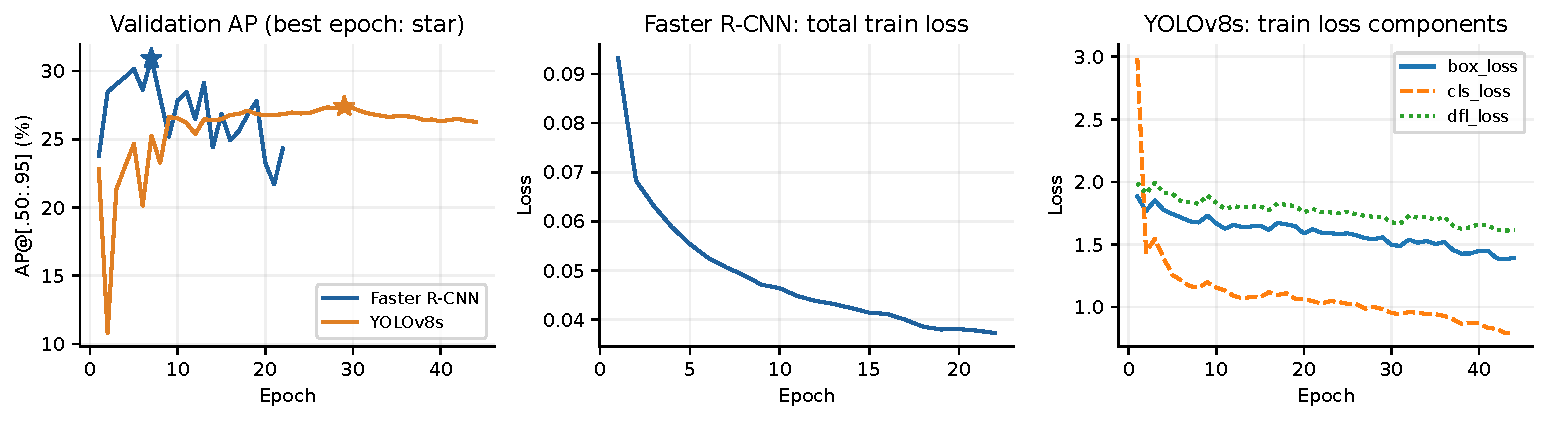
\includegraphics[width=\textwidth]{figures/training.pdf}
\caption{Validation AP và train loss của các run thực tế. Dấu sao là best epoch.
Các loss được vẽ tách panel vì khác định nghĩa/scale; đường loss không dùng để so sánh
trực tiếp chất lượng hai kiến trúc.}
\label{fig:training}
\end{figure*}

\FR{} hoàn thành 22 epoch, best epoch 7, tổng 21.998,54 giây;
\YO{} hoàn thành 44 epoch, best epoch 29, tổng 8.476,35 giây.
Khoảng cách từ best đến cuối đều là 15 epoch, khớp early stopping.
Đây không phải run thất bại vì chưa đạt 100 epoch: 100 là trần ngân sách.
Thời gian lấy từ \texttt{training\_summary.json}; không gồm toàn bộ thời gian tải
dataset/dependency hoặc final test/benchmark của notebook, và không cộng run \FR{}
AMP thất bại trước đó.

\section{Giao thức đánh giá}
\subsection{COCO AP và hậu xử lý thống nhất}
Evaluation dùng pycocotools COCOeval~\cite{coco,cocoeval}, cùng annotation gốc cho cả hai model.
Ngưỡng score floor cho AP là 0,001; NMS IoU 0,5; tối đa 100 detection/ảnh.
YOLO raw head output được giải mã/NMS qua predictor chung, không dùng evaluator native
làm bảng điểm cuối. Tham số NMS native khác trong \texttt{args.yaml} không ghi đè
protocol cuối này. Box đều đưa về pixel ảnh gốc trước khi đánh giá.

IoU giữa hai hộp được xác định bởi
\begin{equation}
 \IoU(A,B)=\frac{|A\cap B|}{|A\cup B|}.
\end{equation}
AP50 và AP75 đo ở IoU 0,50 và 0,75; chỉ số chính lấy trung bình AP qua 10 mức IoU:
\begin{equation}
 \AP=\frac{1}{10}\sum_{k=0}^{9}\mathrm{AP}_{0.50+0.05k}.
\end{equation}
Vì chỉ có một lớp, mAP qua lớp trùng AP của Varroa. AP được tổng hợp theo chuẩn COCO,
không phải accuracy ảnh hoặc AP tại một confidence duy nhất.

\subsection{Threshold, precision, recall và F1}
Threshold vận hành $\tau$ được chọn trên toàn bộ validation bằng F1 lớn nhất ở
IoU 0,5, hòa điểm ưu tiên confidence lớn hơn. Ghép prediction theo score giảm dần,
cùng lớp và cùng ảnh; một ground truth chỉ được nhận tối đa một TP.
Detection trùng hộp đã ghép được tính FP. Các prediction bằng score được xét cùng
mức threshold, tránh chọn ngưỡng không thể thực hiện tại thời điểm inference.
Sau khi chọn, khóa $\tau$ trước khi đọc test predictions.
\begin{align}
 P&=\frac{TP}{TP+FP},\quad R=\frac{TP}{TP+FN},\\
 F_1&=\frac{2PR}{P+R}.
\end{align}
Các giá trị default tìm được là $\tau_F=0,8224449754$ và $\tau_Y=0,2831989825$.
Không so sánh calibration chỉ từ hai số confidence khác nhau; chúng không cùng thang
xác suất đã được hiệu chuẩn. AP vẫn tính ở score floor thấp, không cắt bằng $\tau$
đã chọn cho P/R/F1.

\begin{figure*}[t]
\centering
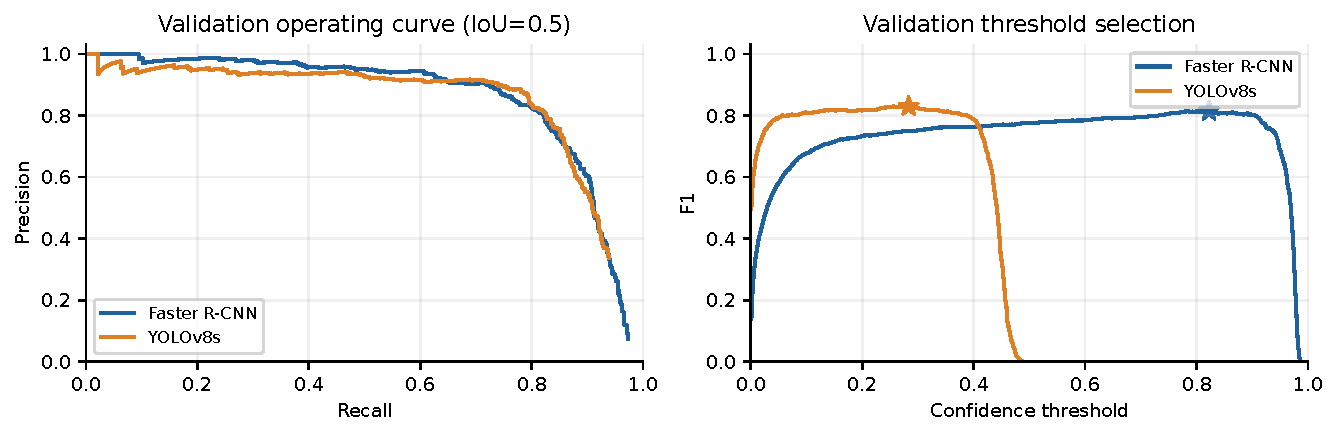
\includegraphics[width=0.96\textwidth]{figures/validation_curves.pdf}
\caption{Đường vận hành precision--recall và F1 theo threshold trên validation,
ghép một-một ở IoU 0,5. Dấu sao chỉ threshold F1 được khóa cho test;
đây không phải đường PR nội bộ của COCO ở mọi mức IoU.}
\label{fig:threshold}
\end{figure*}

Mean IoU TP là trung bình IoU của các hộp được ghép đúng ở threshold trên, cần đọc
cùng recall vì không phản ánh hộp bị bỏ sót. False alarm trên ảnh âm là tỷ lệ ảnh
không có ground truth nhưng có ít nhất một detection; FP/image chia tổng số FP cho
tất cả ảnh. Hai chỉ số này không tương đương vì FP còn có thể xuất hiện trên ảnh dương.

\subsection{Latency và FPS}
Benchmark chạy riêng trên một T4, FP32, batch 1; 20 lượt warmup, 100 ảnh lấy theo
chỉ số đều trên test. Ảnh đã được đọc/giải mã trước phép đo. CUDA được synchronize
trước/sau mỗi mẫu. Phạm vi gồm letterbox, chuyển CPU--GPU, model, NMS, đổi box về
ảnh gốc và chuyển kết quả về CPU; không gồm file I/O/giải mã ảnh.
\begin{equation}
 \mathrm{FPS}=\frac{1000}{\overline{t}_{ms}}.
\end{equation}
Số liệu là throughput suy ra từ latency batch 1, không phải đo video end-to-end,
không gồm vẽ box/UI và không bảo đảm duy trì FPS khi dùng camera thực tế.
VRAM inference là peak tensor allocation của Torch; không phải toàn bộ VRAM do
driver/caching allocator chiếm và không phải yêu cầu GPU tối thiểu khi training.

\section{Kết quả thực nghiệm}
\subsection{Validation và test}
Bảng~\ref{tab:val} cho thấy checkpoint được chọn theo AP, không theo F1.
\FR{} có AP validation tốt hơn nhưng F1 validation thấp hơn \YO{}; đây không phải
mâu thuẫn vì metric và tiêu chí lựa chọn khác nhau.

\begin{table}[t]
\centering\small
\caption{Validation tại best checkpoint và threshold đã chọn.}
\label{tab:val}
\begin{tabular}{lrr}
\toprule
Chỉ số (\%) & Faster R-CNN & YOLOv8s \\
\midrule
AP@[.50:.95] & 30,92 & 27,41 \\
AP50 & 85,78 & 83,39 \\
AP75 & 9,30 & 5,62 \\
Precision & 83,25 & 88,56 \\
Recall & 79,69 & 78,02 \\
F1 & 81,44 & 82,95 \\
\bottomrule
\end{tabular}
\end{table}

\begin{table}[t]
\centering\small
\caption{Test trên 3.408 ảnh, 1.068 ground-truth box. Bảng sinh từ metrics JSON.}
\label{tab:test}
\begin{tabular}{lrr}
\toprule
Chỉ số test & Faster R-CNN & YOLOv8s \\
\midrule
AP@[.50:.95] (\%) & 28,78 & 21,93 \\
AP50 (\%) & 83,43 & 71,16 \\
AP75 (\%) & 8,51 & 5,16 \\
Precision (\%) & 82,00 & 80,15 \\
Recall (\%) & 78,46 & 68,82 \\
F1 (\%) & 80,19 & 74,06 \\
Mean IoU TP (\%) & 68,89 & 67,45 \\
AP small (\%) & 29,98 & 27,15 \\
AP medium (\%) & 29,38 & 20,34 \\
TP & 838 & 735 \\
FP & 184 & 182 \\
FN & 230 & 333 \\
\bottomrule
\end{tabular}

\end{table}

Trên test (Bảng~\ref{tab:test}), \FR{} tăng 6,85 điểm phần trăm AP@[.50:.95],
12,28 điểm AP50, 9,64 điểm recall và 6,14 điểm F1 so với \YO{}.
Precision tăng 1,84 điểm phần trăm. Đây là chênh lệch điểm phần trăm, không nhầm
với phần trăm cải thiện tương đối. Ví dụ AP tăng tương đối khoảng 31,24\%, nhưng
6,85 điểm phần trăm diễn đạt trực tiếp hơn khi so bảng.

\FR{} có 838 TP, 184 FP, 230 FN; \YO{} có 735 TP, 182 FP, 333 FN.
Thêm 103 TP với chỉ thêm 2 FP là lợi thế quan sát được tại hai threshold validation
đã khóa. Tổng TP+FN đều bằng 1.068, phù hợp số ground truth. Test recall vẫn chỉ
78,46\% ở hệ thống tốt hơn: còn khoảng 21,54\% object bị bỏ sót.

\subsection{Localization, kích thước và false alarm}
AP75 chỉ đạt 8,51\% và 5,16\%, thấp hơn nhiều AP50. Mean IoU TP ở IoU 0,5 là
68,89\% và 67,45\%. Các số này cho thấy hạn chế khi yêu cầu box khớp chặt, dù model
thường nhận diện đúng vùng lân cận Varroa ở chuẩn IoU 0,5.
Không quy toàn bộ AP75 thấp cho nhãn thiếu chính xác; cần kiểm toán thêm cả annotation,
độ phân giải nguồn, regressor và hậu xử lý để phân biệt nguyên nhân.

Test có tỷ lệ small box 768/1.068, khoảng 71,91\%. AP small của \FR{} là 29,98\%,
\YO{} 27,15\%; AP medium lần lượt 29,38\% và 20,34\%.
Như vậy, lợi thế AP medium lớn hơn lợi thế AP small trong run này; không dùng kết quả
để khẳng định FPN chỉ cải thiện object nhỏ hay đã chứng minh nhân quả từ kiến trúc.

Trong 2.466 ảnh âm test, \FR{} báo ít nhất một object ở 92 ảnh (3,73\%);
\YO{} ở 38 ảnh (1,54\%). Mặc dù tổng FP gần nhau, phân bố lỗi khác nhau:
\FR{} làm phát sinh cảnh báo trên nhiều ảnh âm hơn. FP/image lần lượt 0,05399 và
0,05340. Nếu ứng dụng tốn công kiểm tra mỗi cảnh báo ảnh, false-alarm-image rate
là chỉ số cần cân nhắc bên cạnh F1.

\subsection{Tốc độ và tài nguyên}
\begin{table}[t]
\centering\small
\caption{Hiệu suất inference với cùng protocol một T4, FP32, batch 1.}
\label{tab:speed}
\begin{tabular}{lrr}
\toprule
Chỉ số & Faster R-CNN & YOLOv8s \\
\midrule
Parameter (triệu) & 41,30 & 11,14 \\
Mean latency (ms) & 67,36 & 19,80 \\
Median (ms) & 67,33 & 19,59 \\
P95 (ms) & 71,20 & 21,62 \\
FPS & 14,84 & 50,51 \\
Peak allocated (MiB) & 365,41 & 89,58 \\
\bottomrule
\end{tabular}
\end{table}

\YO{} nhanh hơn 3,40 lần, có ít hơn khoảng 3,71 lần parameter.
\FR{} có peak VRAM training ghi trong history khoảng 9.387 MiB/GPU (9,17 GiB),
khác rõ với peak inference ở Bảng~\ref{tab:speed} vì training cần activation/gradient
và batch lớn hơn. Artifact YOLO không cung cấp cùng trường peak training tổng hợp
theo protocol này; không điền số ước đoán vào bảng để làm so sánh giả tương đương.

Thời gian training \FR{} dài hơn dù số epoch ít hơn, nhưng không thể giải thích
chỉ bằng kiến trúc: \FR{} dùng FP32, \YO{} AMP và EMA; best/dừng ở epoch khác nhau.
Không dùng thời gian hai run để suy ra một hệ số chậm cố hữu cho mọi thiết lập.

\begin{figure*}[t]
\centering
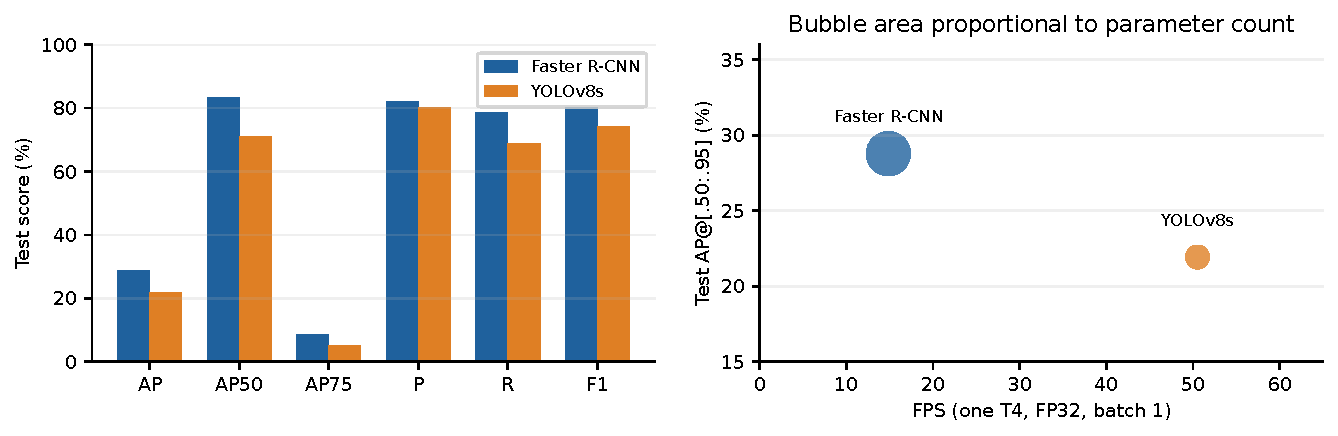
\includegraphics[width=0.96\textwidth]{figures/comparison.pdf}
\caption{So sánh test và accuracy--speed. Diện tích điểm tỷ lệ parameter count.
P/R/F1 dùng threshold riêng đã chọn trên validation; AP dùng protocol COCO chung.}
\label{fig:comparison}
\end{figure*}

\section{Inference trên ảnh mới}
\subsection{Giao diện và đầu ra}
Module \path{inference/predict.py} hỗ trợ một ảnh hoặc thư mục đệ quy, lựa chọn
\texttt{fasterrcnn}, \texttt{yolov8s} hoặc \texttt{both}; device tự chọn CUDA khi có,
nếu không dùng CPU. Notebook \path{inference/inference.ipynb} cho phép cấu hình
source, output, model, device, limit và threshold rồi xem ảnh.

Inference tải \texttt{best.pt}, kiến trúc đúng head và FrozenBatchNorm cho \FR{};
YOLO dùng model/EMA được lưu trong checkpoint. Không tải lại pretrained weights
để thay thế weights fine-tune, không train lại. Ngưỡng được đọc từ
\path{confidence_selection.json}; người dùng có thể override rõ ràng, khi đó phải
coi đây là điểm vận hành mới, không gán các metric đã báo cáo cho threshold khác.

Mỗi model xuất ảnh gốc vẽ box/score, \texttt{predictions.json} theo COCO xywh và
\texttt{run.json} chứa checkpoint, device, precision, threshold, manifest ảnh.
ID trong inference bắt đầu từ 1 và chỉ có ý nghĩa trong lần chạy, không phải ID test
gốc. Ảnh không có prediction vẫn giữ trong manifest. Khi chạy cả hai model, thư mục
\texttt{comparison} chứa hai ảnh cạnh nhau để xem trực quan.

\subsection{Ví dụ sử dụng}
Các lệnh bên dưới chạy từ root repo Lab 3:
\begin{lstlisting}
python inference/predict.py \
  --source /path/to/new_images \
  --model both --device auto

python inference/predict.py \
  --source /path/to/image.png \
  --model fasterrcnn --device cpu
\end{lstlisting}
Pipeline không gọi trực tiếp tiền xử lý default khác của \texttt{YOLO.predict()};
thay vào đó dùng cùng letterbox và predictor với final evaluation để tránh thay đổi
hình học/normalization trong bước triển khai. NMS vẫn là 0,5, max detection 100,
output box được clip trên kích thước ảnh gốc.

\subsection{Kiểm chứng inference}
Đã chạy cả hai checkpoint thật trên 4 ảnh test bằng CPU Torch 2.9.1 và
Torchvision 0.24.1. Số detection khớp artifact Kaggle; chênh lệch box lớn nhất của
\FR{} khoảng $2,29\times10^{-5}$ pixel, của \YO{} khoảng $1,53\times10^{-5}$ pixel;
chênh score YOLO khoảng $2,09\times10^{-7}$, \FR{} bằng 0 trên các detection so khớp.
Đây là smoke check 4 ảnh, không thay thế đánh giá toàn bộ test hoặc bảo đảm mọi
ảnh/GPU đều có kết quả giống bit. Hình inference demo không chứa ground truth.

\section{Phân tích định tính và thảo luận}
\subsection{Trường hợp bổ sung recall và lỗi cảnh báo}
Hình~\ref{fig:qual1} minh họa một ảnh mà \FR{} ghép đúng nhiều object hơn \YO{};
Hình~\ref{fig:qual2} cho thấy cảnh báo trên ảnh được gán negative;
Hình~\ref{fig:qual3} là trường hợp cả hai không ghép đúng Varroa đã được gán nhãn.
Ảnh được chọn bằng quy tắc đầu tiên thỏa từng điều kiện trong thứ tự test gốc,
không chọn theo mức đẹp của hình. Manifest chọn mẫu được lưu để tái hiện.
Mẫu ảnh minh họa không dùng để suy ra tần suất lỗi; tần suất lấy từ toàn bộ test.

\begin{figure}[t]
\centering
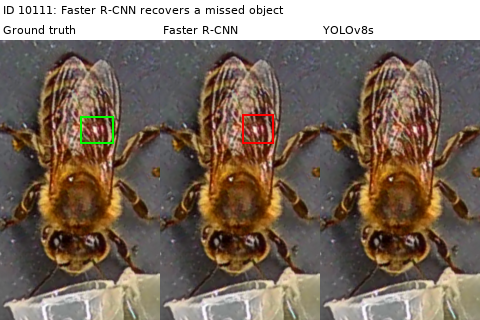
\includegraphics[width=\columnwidth]{figures/qualitative_1.png}
\caption{Mẫu \FR{} thu hồi đối tượng mà YOLO bỏ sót. Trái: ground truth xanh;
giữa: \FR{}; phải: \YO{}, prediction đỏ ở threshold validation riêng.}
\label{fig:qual1}
\end{figure}
\begin{figure}[t]
\centering
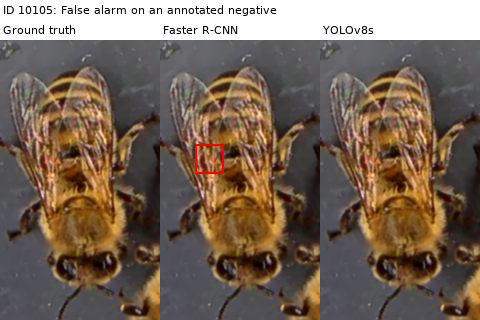
\includegraphics[width=\columnwidth]{figures/qualitative_2.png}
\caption{Một ảnh negative theo annotation có detection của \FR{} và không có
detection YOLO. ``False alarm'' được xác định đối với annotation, không khẳng định
ảnh tuyệt đối không thể chứa đối tượng chưa được gán nhãn.}
\label{fig:qual2}
\end{figure}
\begin{figure}[t]
\centering
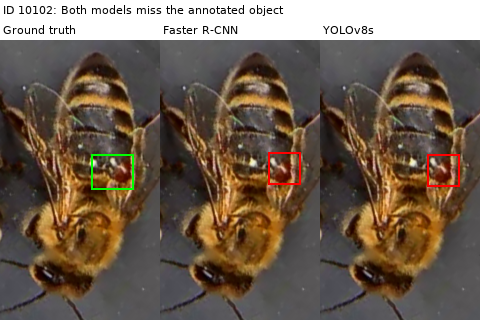
\includegraphics[width=\columnwidth]{figures/qualitative_3.png}
\caption{Một ảnh có Varroa mà cả hai không ghép được TP tại IoU 0,5 và threshold
đã chọn. Hộp dự đoán xuất hiện gần object cũng có thể bị tính FP nếu IoU không đủ.}
\label{fig:qual3}
\end{figure}

\subsection{Overfitting và khoảng cách validation--test}
Với \FR{}, train loss giảm từ 0,0932 xuống 0,0373 nhưng validation AP sau epoch 7
dao động và không vượt 30,92\%; cuối run còn 24,33\%. Đây là dấu hiệu phù hợp với
overfitting hoặc mất hiệu quả tổng quát hóa trong recipe hiện tại; chưa có ablation
để tách tác động learning rate, augmentation và đặc điểm split.
Early stopping cùng best checkpoint tránh dùng weights cuối kém hơn để báo cáo.

Với \YO{}, validation AP tăng dần rồi đạt đỉnh epoch 29, sau đó suy giảm nhẹ trong
khi train loss tiếp tục giảm. Gap AP từ validation sang test của \FR{} là 2,14 điểm,
của \YO{} 5,47 điểm. \YO{} còn đổi thứ hạng F1: cao hơn trên validation nhưng thấp
hơn trên test. Điều này cho thấy threshold chọn ở validation không bảo đảm tối ưu
test, và không được chỉnh threshold bằng test để cải thiện lại số liệu cuối.

\subsection{Lựa chọn hệ thống theo yêu cầu vận hành}
Nếu ưu tiên thu hồi nhiều Varroa hơn trong hai run đã đo, \FR{} là lựa chọn có cơ sở
vì recall, AP và F1 cao hơn. Nếu ưu tiên latency hoặc tài nguyên inference, \YO{}
có lợi thế. Nếu cảnh báo trên ảnh negative gây tốn công kiểm tra, YOLO có tỷ lệ ảnh
false alarm thấp hơn tại điểm vận hành đã khóa. Do đó không có một lựa chọn ``tốt
nhất'' chỉ dựa trên một cột mAP mà bỏ qua chi phí bỏ sót và chi phí cảnh báo.

50,51 FPS của YOLO trong benchmark không tự chứng minh đáp ứng một hệ thống video
thực tế. Cần đo thêm camera, decoding, hàng đợi, vẽ box, độ phân giải khác, nguồn
điện và thermal throttling nếu chuyển sang thiết bị triển khai.

\subsection{Giới hạn khoa học}
Thứ nhất, một seed không đủ ước lượng biến thiên hoặc kiểm định ý nghĩa thống kê.
Thứ hai, pretraining, learning rate, EMA, precision và pipeline riêng của backbone
khác nhau; không coi đây là ablation kiến trúc được kiểm soát tuyệt đối.
Thứ ba, dữ liệu crop trong môi trường kiểm soát chưa chứng minh hiệu quả ngoài hiện
trường, ở camera hay colony khác. Thứ tư, split nguồn có thể còn tương quan phiên quay;
hash/dHash chỉ là bằng chứng chống một số dạng trùng lặp. Thứ năm, evaluation chỉ
dựa vào annotation hiện có; nhãn thiếu hoặc box chưa nhất quán có thể ảnh hưởng số đo.
Thứ sáu, benchmark 100 ảnh không cung cấp phân phối latency cho toàn bộ dữ liệu hoặc
nhiều thiết bị. Không cung cấp confidence interval vì chưa thực hiện ước lượng phù hợp.

\subsection{Hướng phát triển}
Các thực nghiệm tiếp theo nên tách thành giả thuyết kiểm chứng được: chạy nhiều seed;
so sánh ở ngân sách/precision gần nhau; giảm learning rate hoặc thay schedule để
khảo sát overfitting; ablation EMA và augmentation; kiểm toán các case IoU thấp;
đánh giá trên tập ngoài phiên quay. Khảo sát threshold theo chi phí FN/FP hoặc
recall mục tiêu phải thực hiện trên validation, sau đó khóa trước test mới.
Tăng input size không được mặc định là tạo lại chi tiết đã mất ở ảnh nguồn; cần
đo thực nghiệm và so với chi phí latency/VRAM. Chưa có kết quả của các đề xuất này.

\section{Kiểm thử và khả năng tái tạo}
\subsection{Kiểm thử đã thực hiện}
Bộ kiểm thử hiện tại có 17 test pass trên CPU: round-trip box/letterbox; duplicate
detection; empty predictions; oracle COCO; negative samples và batch YOLO; threshold
khi chỉ có FP; metric CSV; DataLoader spawn/smoke subset; final evaluation; \FR{}
forward/backward trên batch trộn dương/âm và batch toàn âm; lỗi loss ở một rank
Gloo làm cả hai rank dừng; cleanup process group; notebook nhúng source; và inference
giữ tọa độ, ảnh rỗng, đường dẫn/filename. Không gọi kiểm thử Gloo CPU là xác nhận
hiệu năng NCCL/T4; bằng chứng GPU là các run Kaggle đã hoàn thành.

Đã đọc lại best/last checkpoint của cả hai model, kiểm tra CRC ZIP/checkpoint;
weights \FR{} đều hữu hạn. Đã kiểm tra hash annotation giữa hai run giống nhau,
đếm lại TP/FP/FN và tính lại AP bằng COCOeval từ exported predictions; kết quả khớp.
Các bước kiểm tra này xác nhận tính nhất quán artifact, không phải một lượt huấn luyện
độc lập hay bảo đảm tất cả lỗi triển khai đều đã bị loại.

\subsection{Tổ chức artifact và tái lập báo cáo}
Repo gồm source, notebook, tests, metadata dữ liệu, predictions, metrics, lịch sử và
report. Dataset ảnh, checkpoint và ZIP nhiều GiB không đưa vào Git; giữ local và
tải lại qua Kaggle nếu cần. LaTeX, hình và bảng được lưu trực tiếp để clean clone
vẫn biên dịch PDF mà không tải checkpoint/dataset.
\path{report/build_figures.py} sinh biểu đồ/bảng từ JSON/CSV; hình định tính cần ảnh
dataset. \path{generated/artifact_sha256.json} lưu hash nguồn số liệu của báo cáo.

Hai run được lưu từ các kernel:
\begin{lstlisting}
kaggle kernels output \
 mthutranhehe/lab3-yolov8 \
 -p output/yolo
kaggle kernels output \
 marcusnguyen007/lab3-faster-r-cnn \
 -p output/faster_r-cnn
\end{lstlisting}
Các đường dẫn download là phương thức lấy artifact đã báo cáo, không phải bằng
chứng rằng run Kaggle tương lai sẽ không bị thay phiên bản bởi chủ kernel.
Hash và metadata local giúp xác định bộ artifact thực tế trong bài này.

\section{Kết luận}
Bài lab hoàn thành pipeline từ kiểm toán VarroaDataset, huấn luyện hai detector đến
evaluation và inference ảnh mới. Trong thiết lập một seed đã đo, \FR{} ResNet50-FPN
đạt AP@[.50:.95] 28,78\%, F1 80,19\%, recall 78,46\% trên test, cao hơn \YO{};
\YO{} đạt 50,51 FPS so với 14,84 FPS của \FR{}. Lợi thế recall của \FR{} đi kèm
chi phí tài nguyên/tốc độ và tỷ lệ ảnh negative bị cảnh báo cao hơn.

Khó khăn chính còn lại là localization ở IoU cao, bỏ sót đối tượng, overfitting và
khả năng tổng quát hóa ngoài điều kiện dữ liệu. Kết quả cung cấp baseline có thể
truy vết, cùng mô-đun inference thống nhất, và không vượt quá bằng chứng của hai run
fine-tune cụ thể trong kết luận về các họ kiến trúc.

\appendix
\section{Danh mục file để kiểm tra kết quả}
Trong mỗi thư mục run: \texttt{config.json} là cấu hình; \texttt{environment.json}
là phiên bản/GPU/hash; \texttt{metrics.json} chứa validation, test và benchmark;
\texttt{comparison.csv} chứa bảy metric chính; \texttt{confidence\_selection.json}
lưu quy tắc/ngưỡng validation; \texttt{test\_predictions.json} và
\texttt{validation\_predictions.json} chứa detection gốc ở score floor.
\texttt{training\_summary.json} lưu thời gian/epoch. History của \FR{} là
\texttt{history.csv}, của YOLO là \texttt{results.csv}.

Với \FR{}, best/last nằm trực tiếp dưới run; với YOLO nằm trong
\texttt{weights/}. Bản lỗi AMP cũ ở \path{buglog/lab3-faster-r-cnn.log}; log của
run thành công nằm trong \path{output/faster_r-cnn/}. Không nhầm hai log này khi
đánh giá trạng thái pipeline.

\section{Lệnh chạy và biên dịch}
Từ root repo Lab 3, cài dependency inference và pytest trong môi trường có cặp
Torch/Torchvision tương thích, rồi chạy:
\begin{lstlisting}
python -m pytest tests -q
python inference/predict.py \
 --source /path/to/images --model both
cd report
make
\end{lstlisting}
PDF dùng XeLaTeX để hỗ trợ Unicode tiếng Việt với font Noto. Nếu không dùng Make,
thứ tự là XeLaTeX, BibTeX rồi XeLaTeX hai lượt. Không cần Internet khi biên dịch
nếu TeX, font và các package đã cài; hình/bảng đã có trong repo.

\bibliographystyle{unsrt}
\bibliography{references}
\end{document}
